\documentclass{article}
\usepackage[utf8]{inputenc} %кодировка
\usepackage[T2A]{fontenc}
\usepackage[english,russian]{babel} %русификатор 
\usepackage{mathtools} %библиотека матеши
\usepackage[left=1cm,right=1cm,top=2cm,bottom=2cm,bindingoffset=0cm]{geometry} %изменение отступов на листе
\usepackage{amsmath}
\usepackage{graphicx} %библиотека для графики и картинок
\graphicspath{}
\DeclareGraphicsExtensions{.pdf,.png,.jpg}
\usepackage{subcaption}
\usepackage{pgfplots}
\usepackage{float}
\usepackage{amssymb}
\usepackage{physics}
\usepackage{listings}
\lstset{language=Java,
        basicstyle=\ttfamily,
        keywordstyle=\color{blue}\ttfamily,
        stringstyle=\color{red}\ttfamily,
        commentstyle=\color{green}\ttfamily,
        morecomment=[l][\color{magenta}]{\#},
        captionpos=b,
        frame=single % рамка вокруг кода
}

\begin{document}
% НАЧАЛО ТИТУЛЬНОГО ЛИСТА
\begin{center}
    \Large
    Федеральное государственное автономное \\
    образовательное учреждение высшего образования \\ 
    «Научно-образовательная корпорация ИТМО»\\
    \vspace{0.5cm}
    \large
    Факультет программной инженерии и компьютерной техники \\
    Направление подготовки 09.03.04 Программная инженерия \\
    \vspace{1cm}
    \Large
    \textbf{Отчёт по лабораторной работе №6} \\
    По дисциплине «Методы оптимизации» (4 семестр)\\
    \large
    \vspace{8cm}

    \begin{minipage}{.33\textwidth}
    \end{minipage}
    \hfill
    \begin{minipage}{.4\textwidth}
    
        \textbf{Студент}: \vspace{.1cm} \\
        \ Дениченко Александр P3212\\
        \textbf{Практик}:  \\
        \ Селина Елена Георгиевна
    \end{minipage}
    \vfill
Санкт-Петербург\\ 2024 г.
\end{center}
\pagestyle{empty}
% КОНЕЦ ТИТУЛЬНОГО ЛИСТА 
\newpage
\pagestyle{plain}


\section*{Задание }
Дано множество из n городов и матрица расстояний между ними. Требуется объехать
все города по кратчайшему пути, причем в каждом городе необходимо побывать один
раз и вернуться в город, из которого был начат маршрут. Задачу необходимо решить с
помощью генетического алгоритма.

\begin{table}[H]
    \centering
    \caption{Исходные данные}
    \begin{tabular}{|c|c|c|c|c|c|}
    \hline
        &Город 1&Город 2&Город 3&Город 4&Город 5\\
        \hline
        Город 1&0&1&1&5&3\\
        Город 2&1&0&3&1&5\\
        Город 3&1&3&0&11&1\\
        Город 4&5&1&11&0&1\\
        Город 5&3&5&1&1&0\\
        \hline
    \end{tabular}
\end{table}
За целевую функцию следует принять сумму расстояний между городами.
Размер популяции N = 4.
Оператор мутации представляет собой случайную перестановку двух чисел в геноме,
которые выбираются случайно. Вероятность мутации 0.01.

\section*{Решение руками}
\begin{table}[H]
    \centering
    \caption{Популяция 1}
    \begin{tabular}{|c|c|c|}
    \hline
    Путь& Значение целевой функции& Вероятность участия в процессе размножения\\
    \hline01234 & 19 & 19/52\\
    01243 & 11 & 11/52\\
    01324 & 17 & 17/52\\
    01342 & 5 & 5/52\\\hline
    \end{tabular}
\end{table}
В качестве родителей выбраны:
\[01243,\ 01324,\ 01234,\ 01342\]
Скрещиваем:
\[012|4|3\ 013|2|4\]
Получили потомки:
\[430|2|1\ 201|4|3\]
Скрещиваем:
\[01|2|34\ 01|3|42\]
Получили потомки:
\[24|3|01\ 34|2|01\]

\begin{table}[H]
    \centering
    \caption{Расширенная популяция}
    \begin{tabular}{|c|c|}
    \hline
    Путь& Значение целевой функции\\
    \hline
    01234 & 19\\
    01243 & 11\\
    01324 & 17\\
    01342 & 5\\
    43021 & 15\\
    20143 & 19\\
    24301 & 11\\
    34201 & 5\\
    
    \hline
    \end{tabular}
\end{table}

\begin{table}[H]
    \centering
    \caption{Популяция 2}
    \begin{tabular}{|c|c|c|}
    \hline
    Путь& Значение целевой функции& Вероятность участия в процессе размножения\\
    \hline
    01342 & 5 & 5/32\\
    34201 & 5 & 5/32\\
    01243 & 11 & 11/32\\
    24301 & 11 & 11/32\\\hline
    \end{tabular}
\end{table}

В качестве родителей выбраны:
\[01342,\ 34201,\ 24301,\ 01243\]

Скрешиваем: \[0|13|42\ 3|42|01\]

Получаем потомков:\[1|42|30\ 4|13|20\]

Скрешиваем: \[24|30|1\ 01|24|3\]

Получены потомки:\[30|24|1\ 24|30|1\]

\begin{table}[H]
    \centering
    \caption{Расширенная популяция}
    \begin{tabular}{|c|c|}
    \hline
    Путь& Значение целевой функции\\
    \hline
    01342 & 5\\
    34201 & 5\\
    01243 & 11\\
    24301 & 11\\
    14230 & 23\\
    41320 & 21\\
    30241 & 13\\
    24301 & 11\\
    
    \hline
    \end{tabular}
\end{table}

\begin{table}[H]
    \centering
    \caption{Популяция 3}
    \begin{tabular}{|c|c|c|}
    \hline
    Путь& Значение целевой функции& Вероятность участия в процессе размножения\\
    \hline
    01342 & 5 & 5/32\\
    34201 & 5 & 5/32\\
    01243 & 11 & 11/32\\
    24301 & 11 & 11/32\\\hline
    \end{tabular}
\end{table}

В качестве родителей выбраны:
\[24301,\ 01243,\ 01342,\ 34201\]

Скрешиваем: \[24|3|01\ 01|2|43\]

Получены потомки: \[30|2|14\ 24|3|01\]

Скрешиваем: \[0|134|2\ 3|420|1\]

Получены потомки: \[1|420|3\ 2|134|0\]

\begin{table}[H]
    \centering
    \caption{Расширенная популяция}
    \begin{tabular}{|c|c|}
    \hline
    Путь& Значение целевой функции\\
    \hline
    01342 & 5\\
    34201 & 5\\
    01243 & 11\\
    24301 & 11\\
    30214 & 15\\
    24301 & 11\\
    14203 & 13\\
    21340 & 9\\
    \hline
    \end{tabular}
\end{table}


\begin{table}[H]
    \centering
    \caption{Популяция 4}
    \begin{tabular}{|c|c|c|}
    \hline
    Путь& Значение целевой функции& Вероятность участия в процессе размножения\\
    \hline
    01342 & 5 & 5/30\\
    34201 & 5 & 5/30\\
    21340 & 9 & 9/30\\
    01243 & 11 & 11/30\\\hline
    \end{tabular}
\end{table}

В качестве родителей выбраны:
\[01243,\ 34201,\ 01342,\ 21340\]

Скрешиваем: \[012|4|3\ 342|0|1\]

Получены потомки: \[431|0|2\ 013|4|2\]

Скрешиваем: \[0|1|342\ 2|1|340\]

Получены потомки: \[3|1|420\ 3|1|402\]

\begin{table}[H]
    \centering
    \caption{Расширенная популяция}
    \begin{tabular}{|c|c|}
    \hline
    Путь& Значение целевой функции\\
    \hline
    01342 & 5\\
    34201 & 5\\
    21340 & 9\\
    01243 & 11\\
    43102 & 5\\
    01342 & 5\\
    31420 & 13\\
    31402 & 21\\
    \hline
    \end{tabular}
\end{table}

\begin{table}[H]
    \centering
    \caption{Популяция 5}
    \begin{tabular}{|c|c|c|}
    \hline
    Путь& Значение целевой функции& Вероятность участия в процессе размножения\\
    \hline
    01342 & 5 & 5/20\\
    34201 & 5 & 5/20\\
    43102 & 5 & 9/20\\
    01342 & 5 & 11/30\\\hline
    \end{tabular}
\end{table}
Получен оптимальный путь: \[01342\] Расстояние: 5

\section*{Машинная реализация алгоритма}

\begin{lstlisting}[caption={GeneticAlgorithm}, breaklines=true, linewidth=\textwidth]
package org.example;

import java.util.*;

public class GeneticAlgorithm {

    private static int[][] graph = {
            {0, 1, 1, 5, 3},
            {1, 0, 3, 1, 5},
            {1, 3, 0, 11, 1},
            {5, 1, 11, 0, 1},
            {3, 5, 1, 1, 0}
    };
    private static final int citiesCount = graph.length;
    private static final int populationSize = 4;
    private static final double mutationProbability = 0.01;
    private static Random random = new Random();

    private static class Way {
        List<Integer> sequence;

        public Way(List<Integer> sequence) {
            this.sequence = new ArrayList<>(sequence);
        }

        public int calculateDistance() {
            int distance = 0;
            for (int i = 1; i < citiesCount; i++) {
                distance += graph[sequence.get(i - 1)][sequence.get(i)];
            }
            distance += graph[sequence.get(citiesCount - 1)][sequence.get(0)];
            return distance;
        }
    }

    public static void main(String[] args) {
        List<Way> population = generateInitialPopulation();
        int currentPopulationNumber = 1;
        int populationCount = 3;

        while (true) {

            if (currentPopulationNumber == populationCount) {
                break;
            }

            List<Way> parents = chooseParents(population);
            List<Way> nextPopulation = createNextPopulation(parents);
            for (int i = 0; i < nextPopulation.size(); i++) {
                Way mutatedChild = mutate(nextPopulation.get(i));
                if (mutatedChild != null) {
                    nextPopulation.set(i, mutatedChild);
                }
            }

            population.addAll(nextPopulation);
            Collections.sort(population, Comparator.comparingInt(Way::calculateDistance));
            if (population.size() > populationSize) {
                population = population.subList(0, populationSize);
            }

            currentPopulationNumber++;
        }

        Way optimalWay = population.get(0);
        System.out.println("Optimal: " + optimalWay.sequence + " Length: " + optimalWay.calculateDistance());
    }

    private static List<Way> generateInitialPopulation() {
        List<Way> population = new ArrayList<>();
        List<Integer> cities = new ArrayList<>();
        for (int i = 0; i < citiesCount; i++) {
            cities.add(i);
        }
        Collections.shuffle(cities);
        do {
            population.add(new Way(new ArrayList<>(cities)));
        } while (nextPermutation(cities) \&\& population.size() < populationSize);
        return population;
    }

    private static boolean nextPermutation(List<Integer> array) {
        int k = array.size() - 2;
        while (k >= 0 \&\& array.get(k) >= array.get(k + 1)) {
            k--;
        }
        if (k == -1) {
            return false;
        }
        int l = array.size() - 1;
        while (array.get(k) >= array.get(l)) {
            l--;
        }
        Collections.swap(array, k, l);
        Collections.reverse(array.subList(k + 1, array.size()));
        return true;
    }

    private static List<Way> chooseParents(List<Way> population) {
        List<Way> parents = new ArrayList<>();
        List<Way> nonChosenWays = new ArrayList<>(population);
        double sumOfDistances = nonChosenWays.stream().mapToDouble(Way::calculateDistance).sum();
        List<Double> cumulativeProbabilities = new ArrayList<>();
        double cumulativeSum = 0;

        for (Way way : nonChosenWays) {
            double probability = way.calculateDistance() / sumOfDistances;
            cumulativeSum += probability;
            cumulativeProbabilities.add(cumulativeSum);
        }

        for (int i = 0; i < populationSize; i++) {
            double r = random.nextDouble() * (cumulativeProbabilities.get(cumulativeProbabilities.size() - 1));
            int chosenIndex = Collections.binarySearch(cumulativeProbabilities, r);
            if (chosenIndex < 0) {
                chosenIndex = -chosenIndex - 1;
            }
            if (chosenIndex >= nonChosenWays.size()) {
                chosenIndex = nonChosenWays.size() - 1;
            }
            parents.add(nonChosenWays.get(chosenIndex));
            nonChosenWays.remove(chosenIndex);
        }
        return parents;
    }


    private static List<Way> createNextPopulation(List<Way> parents) {
        List<Way> nextPopulation = new ArrayList<>();
        for (int i = 0; i < parents.size(); i += 2) {
            Way parent1 = parents.get(i);
            Way parent2 = parents.get((i + 1) % parents.size());
            int breakPoint1 = random.nextInt(citiesCount - 1) + 1;
            int breakPoint2;
            do {
                breakPoint2 = random.nextInt(citiesCount - 1) + 1;
            } while (breakPoint1 == breakPoint2);
            if (breakPoint2 < breakPoint1) {
                int temp = breakPoint1;
                breakPoint1 = breakPoint2;
                breakPoint2 = temp;
            }
            nextPopulation.addAll(crossover(parent1, parent2, breakPoint1, breakPoint2));
        }
        return nextPopulation;
    }

    private static List<Way> crossover(Way parent1, Way parent2, int breakPoint1, int breakPoint2) {
        List<Integer> child1Sequence = new ArrayList<>(Collections.nCopies(citiesCount, -1));
        List<Integer> child2Sequence = new ArrayList<>(Collections.nCopies(citiesCount, -1));
        Set<Integer> takenCities = new HashSet<>();

        for (int i = breakPoint1; i < breakPoint2; i++) {
            child1Sequence.set(i, parent2.sequence.get(i));
            takenCities.add(parent2.sequence.get(i));
            child2Sequence.set(i, parent1.sequence.get(i));
        }

        fillRemainingCities(parent1.sequence, child1Sequence, takenCities, breakPoint1, breakPoint2);
        takenCities.clear();
        fillRemainingCities(parent2.sequence, child2Sequence, takenCities, breakPoint1, breakPoint2);

        return Arrays.asList(new Way(child1Sequence), new Way(child2Sequence));
    }

    private static void fillRemainingCities(List<Integer> parentSequence, List<Integer> childSequence, Set<Integer> takenCities, int breakPoint1, int breakPoint2) {
        int index = 0;
        for (int i = 0; i < breakPoint1; i++) {
            while (takenCities.contains(parentSequence.get(index))) {
                index = (index + 1) % citiesCount;
            }
            childSequence.set(i, parentSequence.get(index));
            takenCities.add(parentSequence.get(index));
        }
        for (int i = breakPoint2; i < citiesCount; i++) {
            while (takenCities.contains(parentSequence.get(index))) {
                index = (index + 1) % citiesCount;
            }
            childSequence.set(i, parentSequence.get(index));
            takenCities.add(parentSequence.get(index));
        }
    }

    private static Way mutate(Way way) {
        if (random.nextDouble() <= mutationProbability) {
            int index1 = random.nextInt(citiesCount);
            int index2;
            do {
                index2 = random.nextInt(citiesCount);
            } while (index1 == index2);
            Collections.swap(way.sequence, index1, index2);
            return new Way(way.sequence);
        }
        return null;
    }
}
\end{lstlisting}

\begin{lstlisting}[caption={Ввод}, breaklines=true, linewidth=\textwidth]
    graph = {{0, 1, 1, 5, 3},
            {1, 0, 3, 1, 5},
            {1, 3, 0, 11, 1},
            {5, 1, 11, 0, 1},
            {3, 5, 1, 1, 0}};
\end{lstlisting}

\begin{lstlisting}[caption={Вывод}, breaklines=true, linewidth=\textwidth]
    Optimal: [0, 1, 3, 4, 2] Length: 5
\end{lstlisting}
\section*{Вывод}
Ознакомился с генетическим алгоритмом и решил задачу с его помощью сначала руками, далее была написана программа, ответ которой сошёлся с ответом, полученным руками.


\end{document}


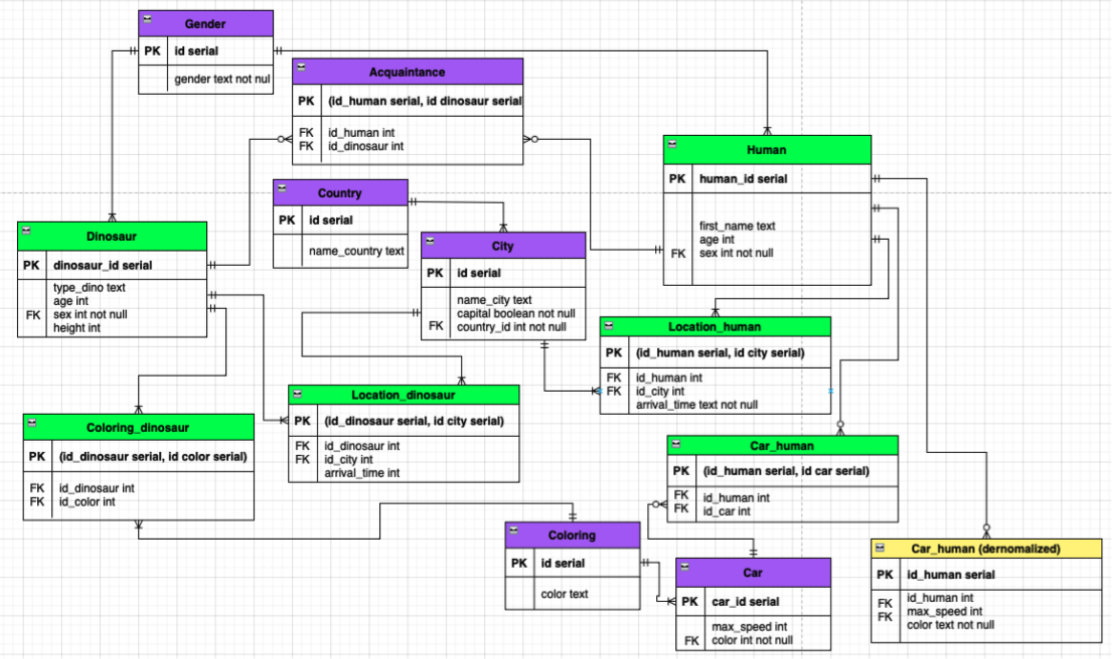
\includegraphics[width=.9\textwidth]{123}



